\section{Estat de l'art}
\label{intro:stateofart}
%El consentiment informat, tal i com s'indica en apartats anteriors, és un procediment, que, tret de comptades ocasions, és d'obligada presència en l'àmbit mèdic.\\
%\newline El procediment actual consisteix en un professional sanitari que informa al pacient de tots els possibles riscos, alternatives al tractament o anàlisis, així com dels possibles beneficis o resultats finals, de forma presencial. Un cop acabada la sessió informativa el pacient rep un contracte on, amb la seva signatura manuscrita afirma, amb ple ús de les seves facultats i sempre de forma totalment voluntària, haver rebut la informació, haver-la comprès i estar-ne d'acord.\\
%\newline Un altre mètode de donar validesa legal, és la signatura electrònica, descrita amb anterioritat. Amb el temps i l'avanç de la tecnologia han aparegut empreses que busquen oferir serveis de certificació i firma electrònica tant a ususaris com a empreses.\\
%\newline Empreses com \textit{Lleida.net\footnote{https://www.lleida.net/}} o \textit{Logalty\footnote{https://www.logalty.com/en/}} operen dins d'Espanya oferint serveis de certificació electrònica a través de la seva plataforma particular o a través d'una API que ells mateixos ofereixen.\\
%\newline El consum dels serveis ofertats per aquestes empreses, les posiciona dins del rol de tercer de confiança, una entitat que actua com un notari online i que, mitjançant un certificat digital i un segell de temps certifiquen que un document ha estat emés en un moment i amb un contingut determinats. 
%\newline Aquest procés, reconegut davant la llei, certifica la integritat del document, així com n'assegura el no repudi.\\
%\newline L'ús de dispositius que capturin traç i pressió també està reconegut per la llei. El principal inconvenient d'aquests dispositius és, deixant de banda la pèrdua de la capacitat d'operar telemàticament, que el seu preu és molt alt, i la seva amortització resulta complicada.\\
%\newline Finalment, a Espanya es disposa de sistemes de certificació com per exemple, el DNI electrònic, que ofereix als usuaris un certificat digital vàl·lid per a autenticar-se i per a signar electrònicament.
%\newline Alternativament, des de ja fa un temps com a complement a l'esmentat e-DNI, existeix \textit{Cl@ve}, un sistema que busca facilitar la identificació dels usuaris davant de l'Administració, alhora que permet signatura electrònica mitjançant certificats.\\
%\newline Els mètodes d'autenticació permesos al sistema \textit{Cl@ve} són mitjançant certificats (e-DNI) o bé mitjançant el que anomenen \textit{Cl@ve PIN}.\\
%\newline Aquest segon mètode, és el que s'anomena contrassenya única o en anglès, \textit{One Time Password} (d'ara en endevant %\textbf{OTP}). L'ús d'aquest mètode es basa en una contrassenya generada a partir de l'instant de temps en el que es sol·licita i, generalment, una clau privada i única de l'usuari, assegurant que per cada usuari i instant de temps, la contrassenya és única, garantint així, la identitat.\\
%\newline Finalment i a mode de conclusió per aquest apartat, vistes les tecnologies anteriors, i entès el problema que es planteja donada la tipologia del negoci de l'empresa, s'ha arribat a la conclusió que existeix la necessitat d'implementar una solució pròpia que satisfagui els requisits particulars de la plataforma en la que en un futur proper s'integrarà al projecte.\\
%\newline Aquesta conclusió ve donada per les "mancances" de les empreses que ofereixen serveis de certificació electrònica presentades anteriorment.\\
%Aquestes mancances resideixen en una necessitat imperiosa de fer passar el procés de certificació per una pàgina web pròpia (de l'empresa certificadora) en la que permeten l'accés al document certificat, provocant d'aquesta forma un canvi de context dins de la plataforma \textit{Made of Genes} que des de l'empresa es considera inacceptable per a l'experiència d'usuari.
\subsection{Genètica i genòmica}
\label{estatArt:genomica_genetica}
Un gen és l'unitat bàsica d'informació biològica que s'implementa físicament sobre una molècula amb unes propietats químiques concretes, que reben el nom d'àcids desoxiribonucleics, altrament coneguts com ADN.\\
\newline L'ADN està format per una cadena nucleòtids que es diferencien els uns dels altres per la seva base nitrogenada, que se solen representar amb quatre lletres:
\begin{itemize}
    \item adenina (A)
    \item citosina (C)
    \item guanina (G)
    \item timina (T)
\end{itemize}
La seqüència d'aquestes quatre lletres (ACGT) serà el que posteriorment es coneixerà com a \textit{genoma}.\\
%\newline Quan parlem de la seqüenciació del \textit{genoma} d'un organisme, ens referim a la seqüència de les bases que trobem en una de les dues cadenes de nucleòtids que formen l'espiral de l'ADN. Només se'n pren una ja que la segona sempre és complementària a la primera.\\
\newline El color dels ulls i de la pell, diferents intoleràncies alimentàries o les propensions a determinades malalties, són característiques que diferencien a un organisme d'un altre i vénen donades per les diferents combinacions de nucleòtids.\\
\newline El conjunt de trets diferencials que mostra un organisme a nivell genètic, rep el nom de \textbf{genotip}, mentre que el conjunt dels seus gens, rep el nom de \textbf{\textit{genoma}}.\\
\newline El \textit{genoma} entre individus de la mateixa espècie pot variar entre ells un 0.1\%.\\
\newline Com a éssers vius, un dels processos genètics que ens caracteritzen, és la rèplica de l'ADN. Aquest procés es realitza milions i milions de vegades al llarg de la vida i es podria assumir com a perfecte.\\
\newline No obstant, no és infal·lible i dóna lloc a mutacions dins de la cadena de l'ADN.\\
\newline Quan ens trobem amb un gen que presenta mutacions a nivell de la seqüència parlem de diferents al·lels.\\
\newline En aquest cas ens trobem amb un gen amb la capacitat de fer la mateixa funció, però amb lleugers canvis. Per exemple, un canvi en la seqüència d’una proteïna pot provocar canvis en la seva eficiència, fent que realitzi la seva funció d'una forma més ràpida o més lenta.\\
\newline Hem anomenat genotip al conjunt de gens present en un individu donat, però com hem vist un mateix gen pot originar trets diferents en funció de diferents factors. Aquesta expressió diferencial del tret l’anomenem \textit{fenotip}, que es pot definir com l’expressió del genotip modulada per la interacció amb el medi.\\
\newline  Així, les dades del nostre genoma parlen sobre la nostra salut present i futura, sobre trets que heredem dels nostres pares i passem als nostres fills i, en general, una informació que pot ser utilitzada per finalitats potencialment discriminatòries. Per això, des de \textit{Made of Genes} es vol donar solució a les problemàtiques inherents a la genòmica, tant a nivell de privacitat com de la tecnologia necessària per la seve anàlisi.\\
\newline Com a curiositat, després d'aquesta breu introducció a la genòmica, cal esmentar que un genoma humà complet pot arribar a ocupar fins a 600GB de dades i que la seva anàlisi pot suposar més de 240 hores càlcul de CPU.\\
%\newline Després d'aquesta breu introducció a la genòmica, podem concloure que les dades que s'extreuen de la seqüenciació del \textit{genoma}, unes dades que parlen directament de qui, que i com és un individu, poden ser considerades extremadament sensibles, i que en determinades circumstàncies podrien ser usades amb fins poc lícits, tals com la discriminació, etc., per això, és necessari un model que garanteixi la privacitat de les dades emmagatzemades. Per satisfer aquesta necessitat, es fa ús d'un sistema de doble encriptació: per una banda, s'encripten les dades amb una clau privada de la pròpia empresa, única per a totes les dades desades, i per l'altre, s'encripten amb un clau única per cada client, que només aquest coneix. D'aquesta forma, s'assegura que en qualsevol cas, si les dades fossin obtingudes sense el permís de l'usuari, no podrien ser des-encriptades de forma convencional.\\
%\newline Per altre banda, a part de l'encriptació, una segona mesura per tal de preservar i garantir la privacitat de les dades és la dividir-les. D'aquesta forma, en cas d'una obtenció no autoritzada de les dades, el que sobté és un segment d'aquestes sense cap mena de relació amb l'anterior bloc de dades, resultant doncs, un bloc poc informatiu per si sol.\\
%\newline Després d'aquesta breu introducció a la genòmica, cal tenir en compte que  unes dades que per si soles parlen de qui, què i com és un individu, venen acompanyades de forma inherent per un seguit de problemàtiques a les que cal buscar sol·lució si el que es busca, és donar sortida a un camp amb un potencial tant gran.\\
%\newline Una primera problemàtica, és que unes dades tant sensibles com les que ens ocupen, podrien ser emprades per exemple, amb intencions discriminatòries, ja no parlem de color de pell ni color dels ulls ni de si un individu és més alt o més baix, si no del cas en que el la informació que ens dóna el seqüenciació, pot revelar certes propensions a una malaltia concreta i això ser usat com a pretext discriminatori cap aquella persona.\\
\newline Lligada a l'obtenció de tot aquest cúmul de dades, però aquests cop lligat als professionals sanitaris, és la possibilitat de descobrir de forma accidental una afecció que poc tingui a veure amb l'estudi o tractament que s'estigui duent a terme. En aquests casos, el professional sanitari està obligat a informar al pacient d'aquesta troballa i en moltes ocasions, pot ser un cas que estigui fora de les competències mèdiques del professional. Aquest fet, aquesta simple por a descobrir quelcom que compliqui el desenvolupament del tractament o estudi, impedeix l'avanç d'una tecnologia o forma de fer les coses que podria beneficiar a tothom.\\
\newline Per aquests motius, l'aposta de \textit{Made of Genes} és la de dividir les dades; tant en la forma de desar-les, com en la forma en la que es donen als especialistes que realitzen les anàlisis.\\
%En el primer dels casos, en cas de que hi hagi una vulneració de les dades i es pogués accedir a les dades emmagatzemades per part de l'empresa, s'accediria a blocs de dades que per si sols poden no tenir cap mena de valor científic i en as de tenir-lo, no revelar la informació sencera, ja que s'hauria de menester d'altres blocs de dades per acabar d'extreure la informació.\\
\newline En el primer dels casos, en el supòsit d'existir una vulneració de les dades emmagatzemades, possiblement es tindria accés a un bloc de dades que de forma individual pot tenir poc valor científic i, en cas de tenir-lo, revelaria poca informació o informació incompleta.
\newline Finalment, pel que respecta a com se serveixen les dades als professionals que realitzen les anàlisis, cada servei té unes dades genòmiques associades necessàries per efectuar l'estudi. Un cop el client autoritza l'ús d'aquestes dades, només es donen al professional
les indicades a l'especificació de l'estudi. Només es serviran les dades genòmiques al complet en el cas que un servei adquirit per un usuari les requereixi.
%\newline Finalment amb la genòmica apareix una problemàtica relacionada amb la informació que és capaç d'aportar.\\
%Es dona el cas de que durant els anàlisis es poden trobar anomalies o detectar possibles problemes en el pacient; i el professional sanitari encarregat de l'anàlisi es veurà obligat a informar del problema sense que aquest sigui molt possiblement del cap d'estudi inicial. Aquest fet, genera cert rebuig cap a un camp com és la medicina personalitzada.\\
%Per a donar solució a la problemàtica, es facilita única i exclusivament la informació necessària per a cada anàlisis, acotant així el possible descobriment de problemes no relacionats amb l'estudi i/o tractament. 

%\newline Així doncs podem dit que en el nostre \textit{genoma} hi ha escrit, per dir-ho d'alguna forma, qui som, les nostres característiques i allò que ens determina, biològicament parlant.\\
%Per un professional sanitari, la informació donaa per la seqüenciació de tot un \textit{genoma}, sovint és innecesària, ja que és més del que bonament necessita per als diagnòstics que desitja realitzar, i al accedir-hi corre el perill de descobrir possibles mutacions que derivin a malalties que no són competència seva però està obligat a manifestr al pacient a qui pertanyen les dades.\\
\subsection{Consentiment informat}
\label{estatArt:consentiment_informat}
%\textbf{Oscar:} \textit{aixó ja ho tens bé, simplement introdueix la problemàtica de que cada petició de servei de made of genes on s'intercanvien un determinat conjunt de dades s'ha d'autoritzar (ho lligues amb els punts anteriors). Posa lo de que sorgeix la problemàtica de la firma a distància si es volen donar a distancia i això t'introdueix el següent punt.}\\
En l'àmbit mèdic, rep el nom de \textit{\textbf{consentiment informat}} el procediment a través del qual es garanteix que, un pacient expressa de forma voluntària la intenció de participar en una investigació o tractament, havent comprès prèviament la informació que se li ha facilitat sobre l'estudi o tractament a realitzar, així com els beneficis, possibles riscos i alternatives, i els seus drets i deures.\\
\newline En ocasions, i en contextos poc rellevants com podria ser un examen físic, aquest consentiment es pot arribar a sobreentendre i no requerir la presència d'un document. No obstant, en procediments invasius, que impliquin cert nivell de risc o bé amb alternatives, el consentiment informat s'ha de presentar per escrit i ha de ser signat pel pacient.\\
\newline Aquest document, serveix per autoritzar a les organitzacions, metges o professionals sanitaris en general, a dur a terme les operacions necessàries amb la seguretat de que el pacient, o la persona sobre la qual recaigui l'efecte del tractament o investigació, n'és conscient.\\
\newline En el cas concret que ens ocupa, el consentiment informat es fa servir per informar, a l'usuari de la plataforma, de tots els detalls referents al servei que sol·licita; però sobretot, l'informa de quina és la informació que cedeix, a qui la cedeix i amb quin propòsit. Per tant, és de vital importància que aquest document estigui present en tota petició de servei que es realitzi a través de la plataforma.\\
\newline Cal recordar que les dades sobre les quals es treballa, són d'un caràcter extremadament sensible i que cada cessió ha d'estar expressament autoritzada pel seu propietari; la qual cosa ens porta a necessitar un sistema per assegurar la conformitat de l'usuari a que es realitzi l'esmentada cessió d'una part, ja sigui global o parcial, de les seves dades genòmiques.\\
\newline Donat el caràcter \textit{on-line} del servei, ens cal un sistema que ens asseguri la conformitat de l'usuari amb tot el procés a l'hora que ens asseguri la seva identitat i ens permeti signar el document, de forma telemàtica; per això es farà ús de la signatura electrònica.

\subsection{Signatura electrònica}
\label{estatArt:signature}
%\textbf{Oscar}: \textit{nou punt, parla de la signatura electrònica, introdueix el tema del OTP-SMS que utilitza la seguretat social i tal, de que hi ha empreses que ho ofereixen (lleida i bla bla bla) i introdueix que el que fan es que actuen com a tercer de confiança}\\

%\textit{A la part de signatura electronica i OTP, no cal que et compliquis. Tu dius "La Ley 59/2003, de 19 de diciembre, de firma electrónica. diu en el seu article 3 que: "10. A los efectos de lo dispuesto en este artículo, cuando una firma electrónica se utilice conforme a las condiciones acordadas por las partes para relacionarse entre sí, se tendrá en cuenta lo estipulado entre ellas." Per tant el que fem es establir un contracte que primer firmen manualment els pacients pero que a partir de llavors firmen mitjançant el seu password. Com que a més a més volem asegurar que el pacient es qui diu ser, fem un doble mecanisme, com fan els bancs o l'estat amb el SMS-OTP. El SMS-OTP, definit en la RFCXXXXX; es basa en el principi que.... I l'expliques per sobre".}\\
\cite{boe} La llei 59/2003 del 19 de desembre sobre signatura electrònica, article 3 paràgraf 10, diu:\\
\newline \textit{"A los efectos de lo dispuesto en este artículo, cuando una firma electrónica se utilice conforme a las condiciones acordadas por las partes para relacionarse entre sí, se tendrá en cuenta lo estipulado entre ellas."}\\
\newline Per tant, en base a aquest article, quan les parts que intervenen en un contracte estan d'acord en la forma en la que es du a terme la signatura del document, aquesta preval per sobre del concepte de signatura que s'especifica al llarg dels 9 punts anteriors.\\
\newline Prenent com a referència un òrgan estatal com és l'administració pública, els mètodes emprats per aquesta a l'hora d'autenticar de forma segura dels seus usuaris i quins mètodes fa servir per la signatura de documents, podem veure que la tendència, és fer ús del sistema \textit{Cl@ve}, que addicionalment al conegut e-DNI, permet autenticar i signar electrònicament mitjançant un sistema anomenat \textit{Cl@ve PIN}.\\
\newline \textit{Cl@ve PIN} és un tipus de codi numèric d'una llargada generalment no inferior a 6 dígits, que pren com a característica principal l'existència d'un temps en el qual pot ser utilitzat, passat aquest temps, se n'haurà de demanar un de nou. Aquest tipus de codi rep el nom de \textit{codi únic} o en anglès, \textit{One Time Password}\cite{otp} (\textbf{\textit{OTP}}).\\
\newline La generacio d'aquests codis OTP, com s'especifica a l'RFC6238, es basa en dos factors:
\begin{enumerate}
    \item Un instant de temps, generalment en format unix time (T).
    \item Un "secret" únic per cada usuari (K).
\end{enumerate}
A grans trets, la generació d'un codi únic basat en un instant de temps, respon a la fórmula: 
\[TOTP = Truncate(K, T)\]
On \textit{Truncate} representa la funció que calcula el codi a partir dels dos factors esmentats anteriorment.\\
Internament parlant, l'algorisme pren aquest instant T, el combina amb el "secret" K de l'usuari i, juntament amb una finestra de temps arbitrària que determina el temps d'utilitat del codi, en genera una seqüència amb \textit{n} dígits, que servirà per a autenticar a l'usuari i certificar-ne la identitat.\\
\newline Veient el model emprat per l'administració pública, hi ha empreses que ofereixen serveis de certificació, validació i signatura de documents, entre altres, seguint els mètodes descrits anteriorment.\\
\newline Aquestes empreses, reben el nom genèric de ``tercer de confiança''.\\
\newline En el cas particular d'aquest projecte, l'usuari signa manualment un primer contracte, amb el qual es queda d'acord en l'ús de la seva contrasenya de la plataforma com a mètode de signatura, i com a mesura de seguretat addicional, ús de codis OTP com a mètode de validació en dos passos.
\subsection{Tercers de confiança, entitats de certificació i nous models}
\label{estatArt:thirdparty}
%\textbf{Oscar}: \textit{Tercers de confiança, entitats de certificació i nou models nou punt, aqui parles del canvi que hi ha des de les entitats de certificació actuals (i expliques els models centralitzats) i com mica en mica es van passant a models distribuïts, on el model per excelencia es:}
Partint de la idea de que el concepte criptografia existeix des de temps molt antics, molt abans de la informàtica, i amb la criptografia, models com el de clau pública-privada (\textit{PKI}) gairebé tan antics com la mateixa criptografia, no es d'estranyar que els principals models de certificació, validació i  signatura estiguin basats en tecnologies amb les que fa anys que convivim. Aquest és el cas de les anomenades "Autoritats de Certificació", entitats reconegudes i de confiança amb la capacitat d'emetre certificats reconeguts i amb validesa legal suficient com per ser irrefutables.\\
\newline Empreses com \textit{Lleida.net}\footnote{http://www.lleida.net/es} o \textit{Logalty}\footnote{https://logalty.com/} decideixen apostar per un model de negoci basat en oferir un servei que permeti la simplificació de processos com la certificació, validació i signatura de documents, fent que tot el procés d'obtenció de certificats i demés sigui transparent a l'usuari.\\
\newline Amb l'aparició d'internet i els sistemes distribuïts, el model \textit{PKI}, un model centralitzat i altament robust i consolidat, en el que es basa tota aquesta infraestructura, ha hagut d'adaptar-se als nous temps, fins i tot ha començat a veure's substituït en ocasions per models que permeten una major flexibilitat o una adaptació major a les necessitats d'aquests nous temps.\\
\newline Dins del marc d'aquest canvi, apareixen tecnologies com \textit{blockchain}, en el que es basa el desenvolupament d'aquest projecte de final de grau.
\clearpage
\subsection{Blockchain}
\label{estatArt:blockchain}
%Blockchain és una estructura de dades ordenada, una llista de blocs de transaccions on cada bloc, es troba ellaçat amb el seu anterior.
%\newline Es pot enmagatzemar en un arxiu de text pla, així com en una base de dades simple. Els “Bitcoin core clients” enmagatzemen les metadades de la blockchain emprant els sistema de base de dades LavelDB de Google. Els blocs tenen un enllaç enrere, fent referència al seu bloc previ dins de la cadena.\\
%\newline Generalment, es visualitza el concepte de blockchain com una pila vertical; la visualització dels blocn empilats, un a sobre de l’altre, resulta en l’ús del terme “height” (alçada) per a referir-se a la distància entre el primer i l’últim bloc, i “top” o bé “tip” per afer referència a l’últim bloc que ha passat a formar part de la blockchain.\\
%\newline Cada bloc dins de la blockchain s’identifica amb un \textit{hash}; aquest es genera mitjançant mitjançant l’algorisme criptogràfic SHA256, a la capçalera. Cada bloc a més, fa referècia a l’anterior, conegut com a “parent block” mitjançant el camp “previous block \textit{hash}” de la capçalera del bloc. En altres paraules, cada bloc conté el \textit{hash} corresponent al seu pare dins de la seva capçalera. la seqüència de \textit{hash} que linquen cada block amb el seu pare, crea una cadena cap enradere fins a arribar al primer bloc creat, conegut com a “genesis block”.\\
%\newline Tot i que un block sols té un pare, temporalment pot tenir multiples fills; cadescún dels fills fa referència al mateix bloc com el seu pare i té el mateix \textit{hash} (el del pare) dins del camp “previous block \textit{hash}” de la seva capçalera. Aquest cas, es dona en el moment que es fa un fork a la blockchain, una situació de caire temporal que es produeix quan es descobreixen diversos blocs de forma simulània per diferents miners.\\
%Finalment, només un dels blocs passarà a formar part de la lockchain, i el “fork” quedarà resolt. Tot i que els blocs puguin tenir un o més fills, cada bloc disposa d’un únic pare. Això es deu a que un bloc té un únic camp “previous block \textit{hash}” referenciant al seu únic pare.\\
%\newline El camp “previous block \textit{hash}” es troba dins de la capcelera del bloc i, afectant directament al \textit{hash} dels blocs fills. La identitat d’un bloc fill canvia si la identitat del pare ho fa; és a dir, quan el pare és modificat, el seu \textit{hash} canvia i inevitablement l’apuntador (“previous block \textit{hash}”) del bloc fill s’ha de modificar amb el nou \textit{hash} del pare. Aquest canvi, alhora provoca que el \textit{hash} del bloc nét es veig també modificat i així succesivament. Aquest efecte cascada asseura que un cop un bloc té diverses generacions que el segueixen, no pot ser canviat sense haver de forçar el recalculat de cadescún dels \textit{hash} dels blocs sunsegüents. Aquest tipus de re-calculat, requereix d’una capacitat de computació molt gran, la existència d’una llarga cadena de blocs fa que la història de la blockchain sigui in-mutable; la qual cosa es converteix en una de les seves principals característiques a nivell de seguretat.

%\subsubsection{Estructura del bloc}
%Un bloc és una estructura de dades que agrega transaccions per a incloure-les a una espècie de llibre de comptes de caràcter públic, la blockchain. El block està format per una capçalera, on es guarden metadades, seguit d’una llarga llista de transaccions (que formen el gruix principal del bloc). \\
%\newline La capçalera ocupa 80 bytes fixes, mentre que una transacció de mitjana pesa com a mínim uns 250 bytes i un bloc de promig conté més de 500 transaccions.\\
%\newline A la següent taula es pot veure més detalladament l'estructura general d'un bloc:
%\begin{table}[ht]
%    \centering
%    \begin{tabular}{|l|l|l|} 
%    \hline
%    \textbf{Mida} & \textbf{Camp} & \textbf{Descripció} \\ [0.2ex] 
%    4 bytes & Block size & La mida del bloc que segueix aquest camp, en bytes \\
%    80 bytes & Block header & Camps corresponents a la capçalera  \\
%    1-9 bytes & Transacion counter & Quantes transaccions segueixen \\
%    Variable & Transactions & Transaccions registrades en el bloc  \\[0.1ex] 
%    \hline
%    \end{tabular}
%    \caption{Estructura general d'un bloc}
%    \label{block_structure}
%\end{table}

%\subsubsection{Capçalera del bloc}
%La capçalera del bloc està formada per tres bloc de metadades: 
%\begin{itemize}
%    \item Un primer bloc amb una referència al \textit{hash} del bloc anterior, que conecta el bloc en qüestió amb el seu anterior dins de la cadena
%    \item  Un segon bloc de metadades que fa referència a temes de mineria de bitcoin
%    \item Un tercer bloc correponent a l’arrel del “merkle tree”, una estuctura de dades per agregar de formaeficient les transaccions del bloc.
%\end{itemize}

%\subsubsection{Identificadors de bloc: \textit{hash} de capçalera i altura del bloc}
%El primer identificador d’un bloc es el seu \textit{hash}, una emprempta digital, generada a partir de realitzar el \textit{hash} (SHA256) de la capçalera 2 vegades. El resultat és un \textit{hash} de 32 bytes anomenat \textit{block \textit{hash}}, tot i que seria més correcte anomenar-lo “block header \textit{hash}”, ja que per a calcular-lo es fa servir únicament la capçalera del bloc. Un \textit{block \textit{hash}} identifica de forma inequívoca i única cada bloc.\\
%\newline Cal notar que aquest \textit{hash} no s’inclou dins del que s’anomena “block’s data structure”, tampoc quan es transmet el block per la xarxa ni quan es persisteix el bloc i passa a formar part de la blockchain. Per contra, cada node calcula aquest \textit{hash} en el moment en el rep el bloc a través de la xarxa. El \textit{block \textit{hash}} es guarda en una base de dades separada com part de les metadades del bloc, per tal de facilitar-ne la indexació i l’accés als bloc del disc.\\
%\newline Una segona forma d’identificar els blocs és mitjançant la seva posició dins de la blockchain, aquesta posició rep el nom d’altura. El primer bloc creat té altura 0. 
%Així doncs, un bloc es pot identificar tant per el seu \textit{block \textit{hash}} o bé per l’altura dins de la blockchain. Cada block afegit sobre aquest primer bloc, afegeix 1 a l’altura de la blockchain. Segons blockchain.info, l’altura de la cadena a data de 21 de Desembre de 2016, és de 444495 blocs, des de gener de 2009.\\
%\newline Cal tenir en compte però, que així com el \textit{block \textit{hash}} és únic per a cada bloc, l’altura no ho és; es poden donar situacions en que més d’un bloc competeixi per la mateixa posició dins de la blockchain. \\
%De la mateixa manera que el \textit{block \textit{hash}}, l’altura és una dada que no forma part de l’estructura de dades del bloc ni s’enmagatzema dins del bloc, sino que cada node calcula de forma dinàmica l’altura del bloc en el moment en el que es rep a través de la xarxa. Igual que el \textit{block \textit{hash}}, l’altura es guarda en una base de dades de metadades.
Una forma de d’entendre la \textit{blockchain}\cite{blockchain} és pensar en un gran llibre de comptes de caràcter públic, on cada transacció que s’efectua queda registrada i on tots els usuaris en tenen accés.
En termes més tècnics, \textit{blockchain} és una llista ordenada, una llista de blocs de transaccions on cada bloc, es troba enllaçat amb el bloc anterior.\\
\newline Generalment, es representa com una pila vertical, per tal d’ajudar a l’hora de definir termes com \textbf{alçada} (\textit{height}), corresponent al total de blocs de la cadena, i al \textbf{\textit{top}}, fet servir per indicar quin es l'últim bloc que ha passat a formar part de la cadena, i que com a conseqüència es troba al cap de munt de la pila representada.\\
\newline Cada bloc dins de la cadena té un identificador, un \textit{hash} generat a partir del contingut de la seva capçalera. Aquest identificador, és el que trobarem dins del camp \textit{previous block hash} del bloc fill.
Seguint els diferents \textit{previous block hash}  de cada element de la cadena, podriem arribar fins al primer bloc, que rep el nom de \textit{genesis block}.\\
\begin{wrapfigure}{r}{0.25\textwidth}
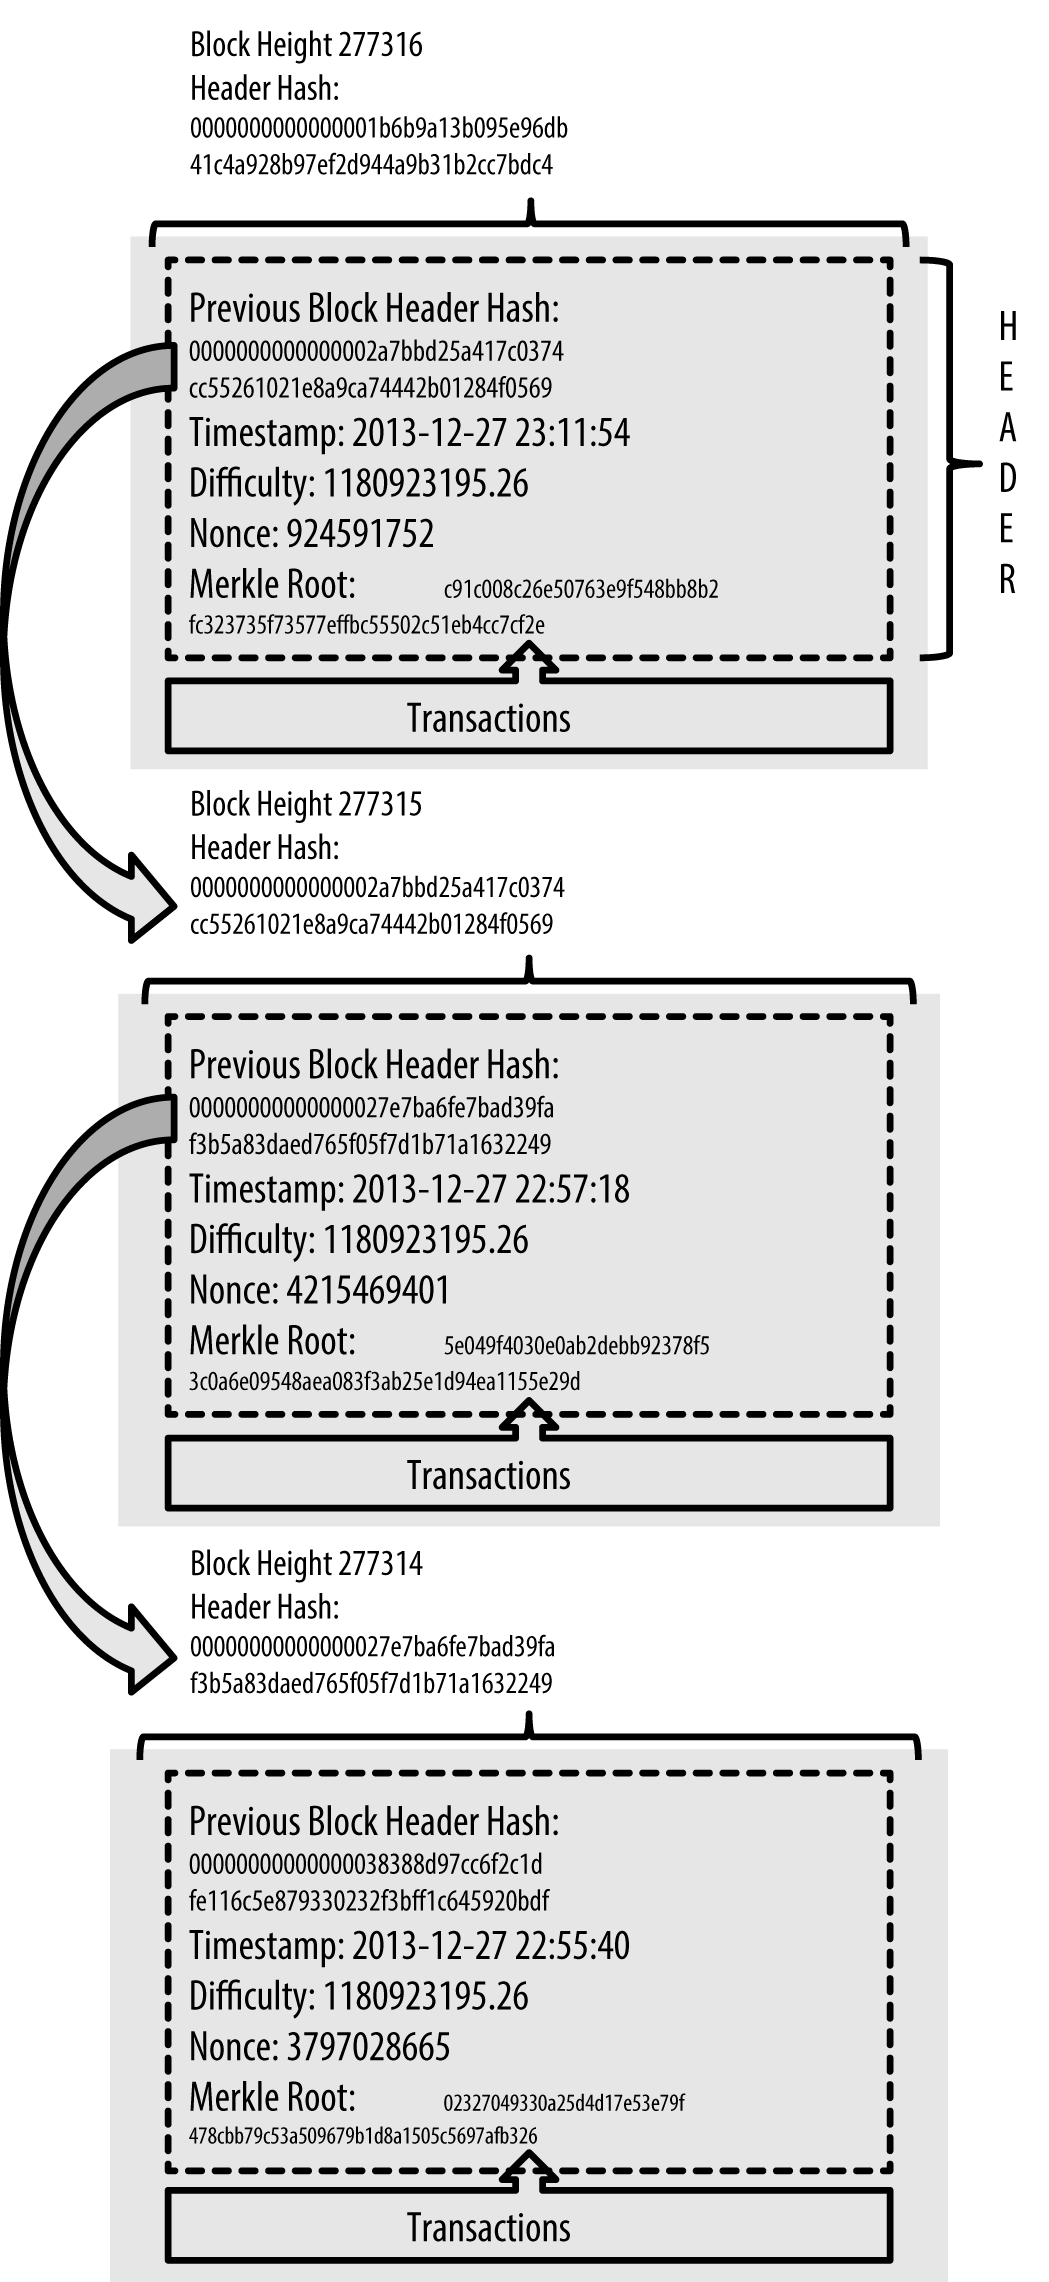
\includegraphics[scale=0.8]{sections/arquitectura/blockchain_diagram.png}
\caption{Blockchain}
\label{fig:blockchain}
\end{wrapfigure}
\newline Una de les característiques principals de \textit{blockchain}, i la que més rellevància té dins del projecte que ens ocupa, és la inmutabilitat de les dades, i en cas de trobar-se un canvi forçós, la facilitat a l’hora de trobar-ne l’origen.\\
\newline Aquesta característica deu el seu origen a la capçalera de cada un dels blocs que formen la cadena.
Dins d’aquesta capçalera, com s'ha dit anteriorment, es troba el camp \textit{previous block hash} que apunta al bloc  anterior, o el que és el mateix, el bloc pare.\\
\newline Fent un resum curt del contingut de la capçalera, trobem aquests tres elements:
\begin{itemize}
    \item Apuntador al bloc anterior (\textit{previous block hash})
    \item Metadades sobre mineria de blocs
    \item \textit{Hash} generat a partir de totes les transaccions registrades al bloc
\end{itemize}
Quan qualsevol dels tres camps que formen la capçalera d’un bloc es veu modificat, l’identificador d'aquest queda modificat, i com a conseqüència, el camp \textit{previous block hash} de la capçalera del fill, fent que l’identificador de bloc del fill es modifiqui, i així successivament fins a replicar-se a tots els nodes de la cadena.\\
\newline Aquesta petita modificació desencadena una successió de canvis a la \textit{blockchain} que requereix d’una capacitat de càlcul molt gran, i és fàcilment detectable.